\documentclass{beamer}
  \usepackage[utf8]{inputenc}
  \usetheme{Warsaw}
  \graphicspath{images/}
  \usepackage{amsmath} 
  \usepackage{amssymb}

  \title{New Technologies are causing problems for society?}
  \author{Clément CAUMES \& Mehdi MTALSI-MERIMI}
  \institute{UFR des Sciences Versailles - M1 Informatique}
  \date{
  	\begin{itemize}
  		\setbeamertemplate{itemize item}[default]
  		\item Introduction
  		\item Environmental impact of the new technologies (resources and pollution)
  		\item Social impact of the new technologies (addiction, inequalities and conflicts) 
  		\item Conclusion
  	\end{itemize}
  } % RAJOUTER PLAN ICI

  \begin{document}

\section{Introduction}

  \begin{frame}
  \titlepage
  \end{frame}

\section{A curb for our planet}

\subsection{Destroy resources}

 \begin{frame}
\begin{block}{Issues of resources} 
	Increase of population, demands and productions induce :
	\begin{itemize}
		\setbeamertemplate{itemize item}[circle]
		\item Resource overexploitation
		\item Extinction of rare animals and plant species
	\end{itemize}
	\hspace{2.5cm}
	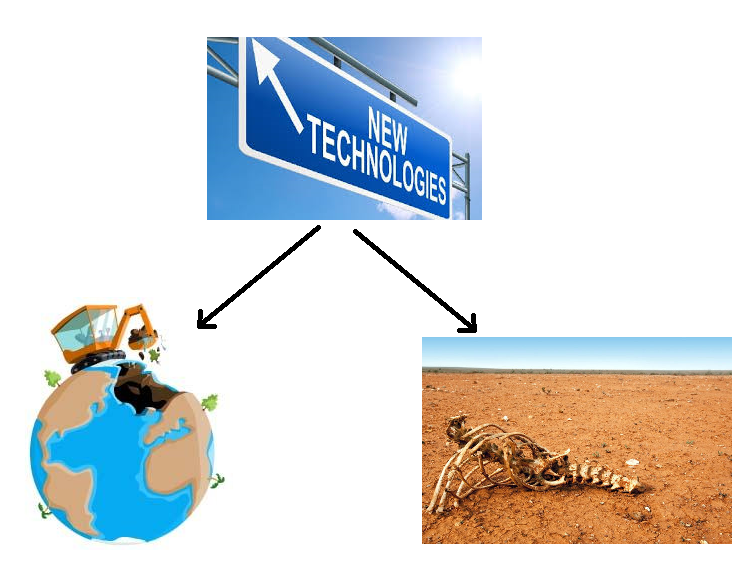
\includegraphics[scale=0.3]{pics/image1.png}
	\end{block}
\end{frame}

\begin{frame}

\begin{block}{Date of exhaustion of mineable resources} 
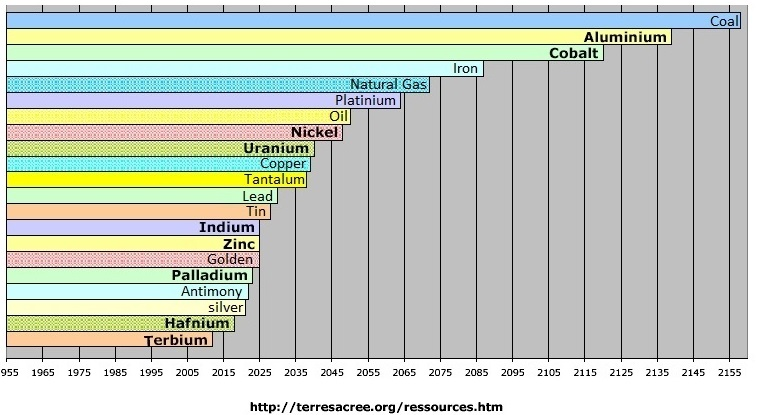
\includegraphics[scale=0.40]{pics/image2.jpg}
\end{block}

\end{frame}

\subsection{Contribute to the pollution}

 \begin{frame}
\begin{block}{Sustainable development = solution ?} 
	\begin{itemize}
		\setbeamertemplate{itemize item}[circle]
		\item Development of the economy
		\item Development of the social aspect
		\item Preservation of the environment
	\end{itemize}
	\hspace{2.5cm}
	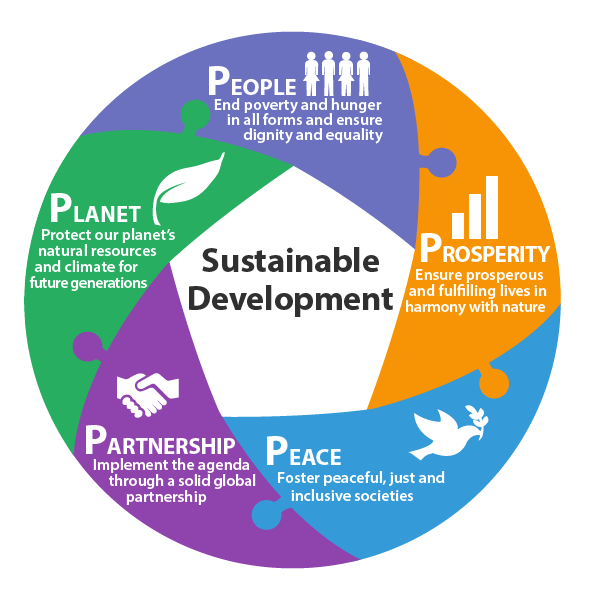
\includegraphics[scale=0.2]{pics/image3.png}
\end{block}
\end{frame}

 \begin{frame}
\begin{block}{Emissions of fossil carbon since 1800} 
	\hspace{4cm}
	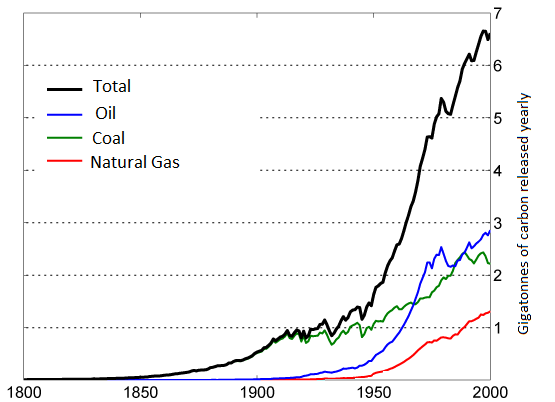
\includegraphics[scale=0.6]{pics/image5.png}
\end{block}
\end{frame}


\section{An impact for a social perspective}

\subsection{Increase addictions}

 \begin{frame}
\begin{block}{Addiction of new technologies} 
	\begin{itemize}
		\setbeamertemplate{itemize item}[circle]
		\item New technologies change the behaviour of young people
	\end{itemize}
	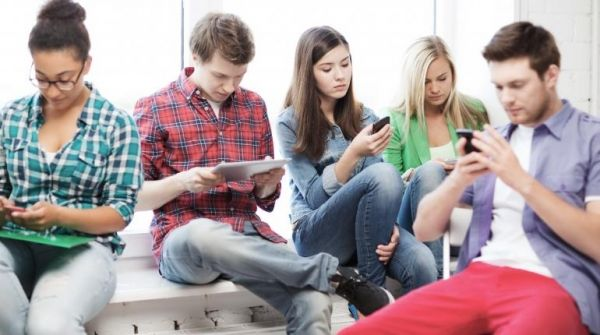
\includegraphics[scale=0.5]{pics/image6.jpg}
\end{block}
\end{frame}

\subsection{Create Inequalities}

 \begin{frame}
\begin{block}{Poverty vs Wealth} 
	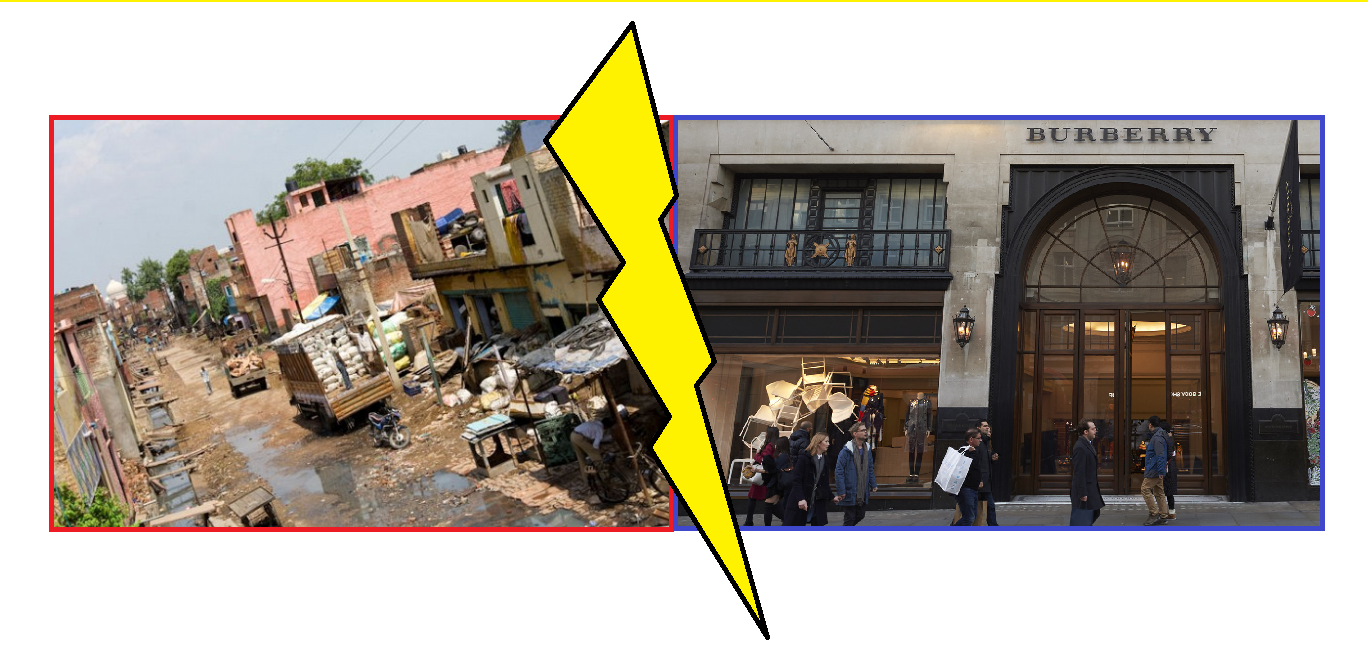
\includegraphics[scale=0.3]{pics/image7.png}
\end{block}
\end{frame}

\subsection{Create Conflicts}

 \begin{frame}
\begin{block}{Authority due to the new technologies} 
	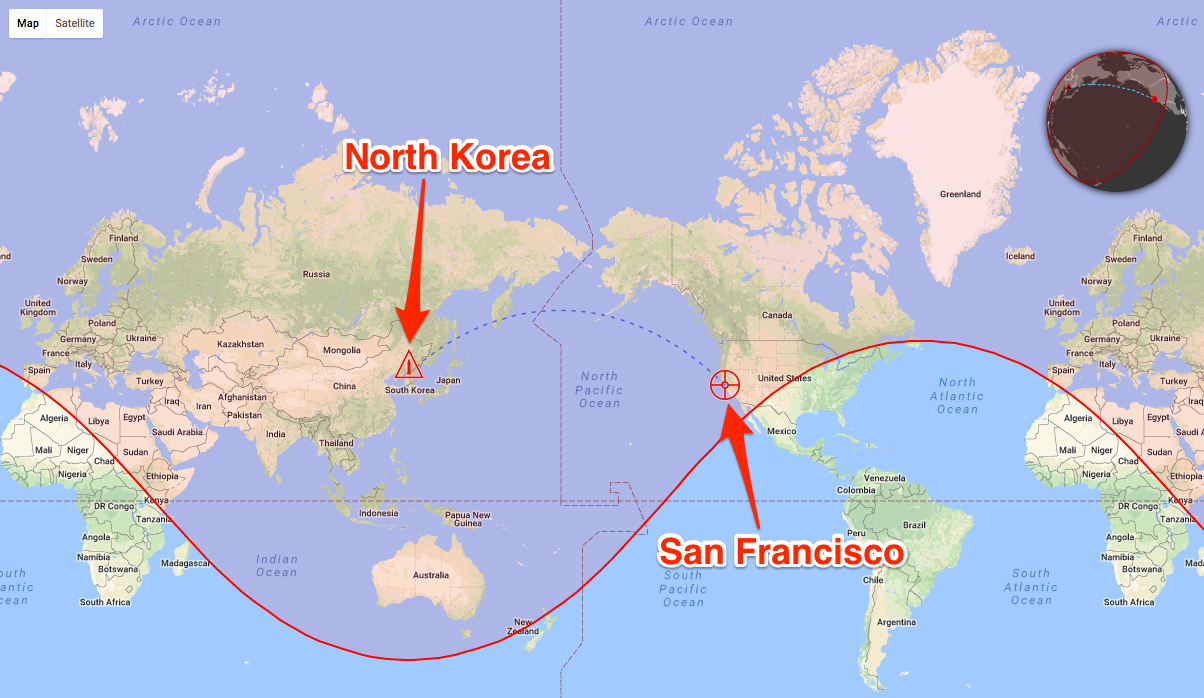
\includegraphics[scale=0.25]{pics/image8.png}
\end{block}
\end{frame}

\section{Conclusion}

 \begin{frame}
\begin{block}{Are New technologies (NT) an issue for society?} 
	\begin{itemize}
		\setbeamertemplate{itemize item}[circle]
		\item NT $\Rightarrow$ Increase Production $\Rightarrow$ Resources emptied
		\item NT $\Rightarrow$ Addiction
		\item NT $\Rightarrow$ Inequalities
		\item NT $\Rightarrow$ Conflicts
	\end{itemize}
\end{block}
\end{frame}

\section{References}

 \begin{frame}
\begin{block}{What were our references?} 
	\begin{itemize}
		\setbeamertemplate{itemize item}[circle]
		\item \textcolor{red}{Resources emptied :} \footnotesize \url{http://terresacree.org/ressources.htm} \normalsize
		\item \textcolor{red}{Sustainable Development :} \footnotesize \url{https://sustainabledevelopment.un.org/?menu=1300} \normalsize
		\item \textcolor{red}{Pollutante emissions :} \footnotesize \url{http://www.sequovia.com/actualites/2075-un-bilan-complet-du-changement-climatique-actuel.html}
		\normalsize
		\item \textcolor{red}{Addictions :} \footnotesize
		\url{https://www.cbc.ca/radio/thesundayedition/the-sunday-edition-november-19-2017-1.4406916/what-are-smartphones-doing-to-young-people-1.4406942} \normalsize
		\item \textcolor{red}{Inequalities :} \footnotesize \url{https://commons.com.ua/en/novi-tehnologiyi-i-globalna-nerivnist/} \normalsize
		\item \textcolor{red}{Conflicts :} \footnotesize
		\url{https://www.lejournalinternational.fr/New-Technologies-for-New-Conflicts_a2804.html} \normalsize
	\end{itemize}
\end{block}
\end{frame}
      
\end{document}
